\documentclass[a4paper, 12pt]{article}

\usepackage{arxiv}

\usepackage[utf8]{inputenc}
\usepackage[english, russian]{babel}
\usepackage[T2A]{fontenc}
\usepackage{cmap}
\usepackage{url}
\usepackage{booktabs}
\usepackage{nicefrac}
\usepackage{microtype}
\usepackage{lipsum}
\usepackage{graphicx}
\usepackage{natbib}
\usepackage{doi}
\usepackage{multicol}

%% Шрифты
\usepackage{euscript} % Шрифт Евклид
\usepackage{mathrsfs} % Красивый матшрифт

\usepackage{amsmath,amsfonts,amssymb,amsthm,mathtools,dsfont}
\usepackage{icomma}

\newcommand{\bz}{\mathbf{z}}
\newcommand{\bx}{\mathbf{x}}
\newcommand{\by}{\mathbf{y}}
\newcommand{\bw}{\mathbf{w}}
\newcommand{\bfx}{\mathbf{f}}
\newcommand{\bb}{\mathbf{b}}
\newcommand{\bu}{\mathbf{u}}
\newcommand{\bX}{\mathbf{X}}
\newcommand{\bZ}{\mathbf{Z}}
\newcommand{\bH}{\mathbf{H}}
\newcommand{\bA}{\mathbf{A}}
\newcommand{\bI}{\mathbf{I}}
\newcommand{\bJ}{\mathbf{J}}
\newcommand{\bV}{\mathbf{V}}
\newcommand{\bU}{\mathbf{U}}
\newcommand{\bG}{\mathbf{G}}
\newcommand{\btheta}{\boldsymbol{\theta}}
\newcommand{\bPsi}{\boldsymbol{\Psi}}
\newcommand{\bpsi}{\boldsymbol{\psi}}
\newcommand{\bxi}{\boldsymbol{\xi}}
\newcommand{\bchi}{\boldsymbol{\chi}}
\newcommand{\bzeta}{\boldsymbol{\zeta}}
\newcommand{\blambda}{\boldsymbol{\lambda}}
\newcommand{\beps}{\boldsymbol{\varepsilon}}
\newcommand{\bZeta}{\boldsymbol{Z}}
% mathcal
\newcommand{\cX}{\mathcal{X}}
\newcommand{\cY}{\mathcal{Y}}
\newcommand{\cW}{\mathcal{W}}

\newcommand{\dH}{\mathds{H}}
\newcommand{\dR}{\mathds{R}}
% transpose
\newcommand{\T}{^{\mathsf{T}}}

\renewcommand{\shorttitle}{\textit{arXiv} Шаблон}
\renewcommand{\epsilon}{\ensuremath{\varepsilon}}
\renewcommand{\phi}{\ensuremath{\varphi}}
\renewcommand{\kappa}{\ensuremath{\varkappa}}
\renewcommand{\le}{\ensuremath{\leqslant}}
\renewcommand{\leq}{\ensuremath{\leqslant}}
\renewcommand{\ge}{\ensuremath{\geqslant}}
\renewcommand{\geq}{\ensuremath{\geqslant}}
\renewcommand{\emptyset}{\varnothing}

\usepackage{hyperref}
\usepackage[usenames,dvipsnames,svgnames,table,rgb]{xcolor}

\hypersetup{
	unicode=true,
	pdftitle={A template for the arxiv style},
	pdfsubject={q-bio.NC, q-bio.QM},
	pdfauthor={David S.~Hippocampus, Elias D.~Striatum},
	pdfkeywords={First keyword, Second keyword, More},
	colorlinks=true,
	linkcolor=black,        % внутренние ссылки
	citecolor=blue,         % на библиографию
	filecolor=magenta,      % на файлы
	urlcolor=blue           % на URL
}

% \usepackage{csquotes} % Еще инструменты для ссылок
\usepackage{enumitem} % Для модификаций перечневых окружений (itemize, list, ...)
\renewcommand{\abstractname}{Аннотация}

\title{Восстановление траектории движения руки по видео}

\author{Владимиров Эдуард \\
	\texttt{vladimirov.ea@phystech.edu} \\
	
	\And
	Курдюкова Антонина \\
	\texttt{kurdiukova.ad@phystech.edu} \\

	\And
	Исаченко Роман \\
	\texttt{roman.isachenko@phystech.edu} \\
	
	\And
	Стрижов Вадим \\
	\texttt{strijov@ccas.ru}
}
\date{\today}

\begin{document}
\maketitle

\begin{abstract}
	В работе решается задача прогнозирования временного ряда со сложной структурой. Под сложной структурой понимается наличие нелинейных зависимостей и варьирующийся период. Требуется найти причинно-следственные связи между временными рядами. Для этого предлагается снизить размерность траекторных пространств. В работе показано, что методы канонического корреляционного анализа, такие как метод главных компонент, метод частичных наименьших квадратов и другие, являются частным случаем метода перекрестных отображений Сугихары. Для демонстрации результатов работы решается задача восстановления траектории движения руки по видео.
\end{abstract}


\keywords{временной ряд \and фазовая траектория \and траекторное подпространство \and сходящееся перекрёстное отображение \and частичные наименьшие квадраты \and канонический корреляционный анализ}

\section{Введение}

В данной работе решается задача прогнозирования временного ряда на основе других временных рядов. 
Одна из трудностей задачи заключается в обнаружении связи между временными рядами и исключении несвязанных временных рядов из прогностической модели. 
Решение этой проблемы повышает её качество.

В данной работе применяется метод сходящегося перекрёстного отображения (convergent cross mapping, CCM) \citep{Sugihara90, sugihara1990nonlinear}, который эффективен для временных рядов, порождённых динамической системой. 
Он основан на сравнении ближайших соседей в траекторном пространстве временного ряда $\bx$, полученных с помощью ряда $\by$.

При построении прогностической модели используется траекторная матрица (или матрица сдвига), описывающая фазовое пространство временного ряда. 
Например, в методе анализа спектральных компонент (singular spectrum analysis, SSA) \citep{golyandina2005ssa, golyandina2001analysis, zhigljavsky2010singular} прогноз временного ряда основан на спектральном разложении ковариационной матрицы, полученной по траекторной матрице. 
В CCM матрицы сдвига используются для проверки наличия липшицева отображения между траекторными пространствами.

Однако размерность траекторного пространства может оказаться чрезмерно высокой, что приводит к неустойчивости прогностической модели.
В таком случае необходимо снизить размерность траекторного пространства путём построения проекции фазовой траектории в некоторое подпространство. Для CCM нет конкретного способа выбрать подпространство, в котором аппроксимируется фазовая траектория.
В работе \citep{usmanova2020sphere_regr} эта проблема решается с помощью сферической регрессии. Согласно этому методу, информация об искомом подпространстве извлекается из множества эмпирических направлений $\{ \bx_i - \bx_j\, | \, i < j \}$.
В работе \citep{alexandrov2005automatic} используется автоматический выбор пары главных компонент. Идея заключается в сравнении спектральных плотностей главных компонент. Также используется простой перебор по главным компонентам \citep{usmanova2019dependencies}.

Метод проекции в латентное пространство (partial least squares, PLS) \citep{rosipal2011nonlinear, rosipal2005overview} отбирает наиболее значимые признаки и строит новые как их линейные комбинации. 
Это позволяет получить простую, точную и устойчивую прогностическую модель.
Наряду с PLS используется метод канонического анализа корреляции (canonical correlation analysis, CCA) \citep{hardoon2004canonical}. 
Он похож на PLS за исключением того, что первый метод максимизирует ковариацию между проекциями, а последний ~--- корреляцию. 
Недостатком этих моделей является их низкая точность при оценивании нелинейных зависимостей между данными.
Разработаны нелинейные модели PLS \citep{qin1992nonlinear} и CCA \citep{andrew2013deep}.
В данной статье используется модель NNPLS \citep{bulut2014new}, которая преобразует исходные данные с помощью нейронной сети. 

В теоретической части работы показано, что методы снижения размерности CCA и PLS являются частными случаями CCM. 
Для этого вводятся различные меры близости между целевой переменной и её аппроксимацией; при этом она является линейной комбинацией её ближайших соседей. 
% для сравнения качества согласованности исходного пространства и его подпространства.

В качестве модели для предсказания временного ряда по набору временных рядов используется алгоритм локально взвешенного глобального линейного отображения (sequential locally weighted global linear map, SMap) \citep{sugihara1994nonlinear}.

Эксперимент проводится на наборе собранных вручную данных. Он представляет собой совокупность ключевых точек, полученных 
по видео движения человека, а также показания акселерометра и гироскопа, снятые с руки человека. 
В эксперименте строится прогноз временных рядов, использующий обнаруженные связанные компоненты временных рядов.

\section{Постановка задачи}
Пусть значения исходного временного ряда $\bx(t)$ доступны в  моменты времени $t = 1, 2, \ldots, n$. Предполагается, что на значения $\bx(t)$ оказывает влияние набор временных рядов $\by_1(t), \ldots, \by_m(t)$.

Для прогноза в момент времени $n$ необходимо определить будущие значения исходного временного ряда $\bx(t)$ в моменты времени $n+1, \ldots, n+p$, учитывая влияние внешних факторов $\by_1(t), \ldots, \by_m(t)$. При этом предполагается, что значения внешних факторов являются доступными в моменты времени: \[\by_1(n+1), \ldots, \by_1(n+p), \ldots, \by_m(n+1), \ldots, \by_m(n+p).\]

Для вычисления будущих значений временного ряда требуется определить функциональную зависимость, отражающую связь между прошлыми значениями $\bx$ и будущими, а также принимающую во внимание влияние внешних факторов $\by_1, \ldots, \by_m$.

\begin{definition}
	\textbf{Моделью прогнозирования с учётом внешних факторов} называется функция:
	\begin{equation*}
		\bx(t) = F(\bx(t-1), \ldots, \by_1(t), \, \by_1(t-1), \ldots, \by_m(t), \, \by_m(t-1), ...) + \epsilon_t.
	\end{equation*}
\end{definition}

Требуется создать такую модель, для которой среднее квадратичное отклонение истинного значения от прогнозируемого стремится к минимальному для заданного $p$. 

\begin{equation*}
	\widehat{E} = \dfrac{1}{p} \sum\limits_{i=n+1}^{n+p} \epsilon_i^2 \rightarrow \underset{F}{\text{min}}.
\end{equation*}

\subsection{Метод CCM}
\begin{figure}[bhtp]
	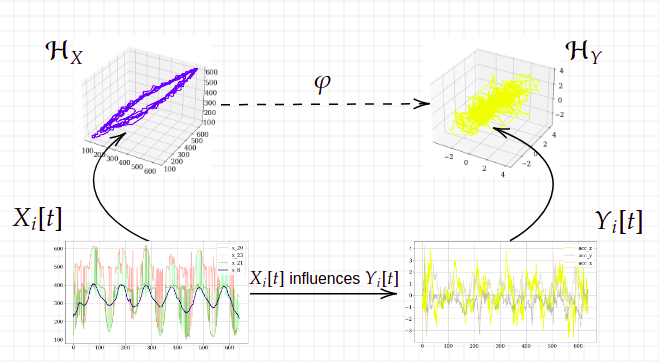
\includegraphics[width=\textwidth]{block_scheme_2.png}
	\caption{Блок-схема}
	\label{fig:schema}
\end{figure}

Определим траекторную матрицу временного ряда $\bx = [x_1, \ldots, x_n]$ следующим образом: 

\begin{equation*} \label{eq:traj_mat}
	\bH_{\bx} = \begin{bmatrix}
		x_1 & x_2 & \ldots & x_{\tau} \\
		x_2 & x_3 & \ldots & x_{\tau+1} \\
		\vdots & \vdots & \ddots & \vdots \\
		x_{N} & x_{N+1} & \ldots & x_n
	\end{bmatrix}, 
\end{equation*} 

где $N$ --- число задержек, $\tau = n - N + 1$.

Обозначим $i\text{-ый}$ столбец матрицы $\bH_{\bx}$ за $\bx_i$. 
Матрица $\bH_{\bx}$ принимает вид:

\begin{equation*} \label{eq:traj_mat_short}
	\bH_{\bx} = [\bx_1, \ldots, \bx_{\tau}], \qquad \bx_i = [x_i, x_{i+1}, \ldots, x_{i+N-1}]\T 
\end{equation*}

Заметим, что все векторы $\bx_t$ принадлежат $N\text{-мерному}$ траекторному пространству $\dH_{\bx} \subseteq \dR^N$ ряда $\bx$ и образуют фазовую траекторию $\bx(t) \in \dR^N$.

Для обнаружения зависимости между временными рядами $\bx$ и $\bz$ возьмём элемент $\bx_0$ из траекторного пространства $\dH_{\bx}$ и найдём $k$ ближайших соседей в этом же пространстве. Обозначим их временные индексы (от ближнего к дальнему) $t_1, \ldots, t_k$.

Так как оба временных ряда определены на одной временной оси, то по значению временного ряда $\bx$ в момент времени $t_0 \in \{ 1, \ldots, n\}$ можно однозначно получить значение временного ряда $\bz$ в тот же момент времени, и наоборот. Введём отображение из $\dH_{\bx}$ в $\dH_{\bz}$ следующим образом: 
$$ \phi: \bx_0 \mapsto \widehat{\bz_0} = \sum\limits_{i=1}^k w_i \bz_{t_i}, \qquad 
w_i = \dfrac{u_i}{\sum\limits_{j=1}^k u_j}, \qquad
u_i = \exp(-||\bx_0 - \bx_{t_i}||).$$

\begin{definition}
	Будем считать временные ряды $\bx$ и $\bz$ \textbf{связанными}, если отображение $\phi$ является липшицевым:
	$$ \rho_{\dH_{\bz}}(\phi(\bx_i), \phi(\bx_j)) \leq C \rho_{\dH_{\bx}}(\bx_i, \bx_j) \qquad \bx_i, \bx_j \in \dH_{\bx}. $$
\end{definition}

Для проверки наличия связанности введём меру близости векторов в окрестностях $U_k(\bx_{t_0})$ и $U_k(\bz_{t_0})$:

\begin{equation}
	L(\bx, \bz) = \dfrac{R(U_k(\bx_{t_0}))}{R(U_k(\bz_{t_0}))}, \qquad R(U_k(\bx_{t_0})) = \dfrac{1}{k} \sum\limits_{i=1}^k \rho_{\dH_{\bx}}(\bx_{t_0}, \bx_{t_j}).
\end{equation}

Если $L(x, z)$ больше некоторого порога $C(n)$, то временной ряд $\bz$ зависит от временного ряда $\bx$.

% Предполагается, что размерность траекторного пространства избыточна, что приводит к неустойчивости прогностической моделей ряда $\bx$.
% Поэтому предлагается рассматривать не саму траекторию $\bx(t)$, а ее проекцию $$\bx_l(t) \in \dR^l, \; l < N$$ в траекторное подпространство 

\subsection{Метод PLS}
Метод частичных наименьших квадратов восстанавливает связь между наборами данных $\bX$ и $\bY$. 
Матрицы объектов $\bX$ и целевая матрица $\bY$ проецируются на латентное пространство $\dR^l$ меньшей размерности следующим образом:
$$ \underset{n \times m}{\bX} = \underset{n \times l}{\bT} \cdot \underset{l \times m}{\bP\T} + \underset{n \times m}{\bE} $$
$$ \underset{n \times k}{\bY} = \underset{n \times l}{\bU} \cdot \underset{l \times k}{\bQ\T} + \underset{n \times k}{\bF}, $$
где $\bT$ и $\bU$ --- матрицы описания объектов и исходов в латентном пространстве, $\bP$ и $\bQ$ --- матрицы перехода из латентного пространства в исходное, $\bE$ и $\bF$ --- матрицы остатков.

Псевдокод метода регрессии PLS приведен в алгоритме \ref{alg:pls}. Алгоритм итеративно на каждом из $K$ шагов вычисляет по одному столбцу $\bt_k, \bu_k, \bp_k, \bq_k$ матриц $\bT, \bU, \bP, \bQ$ соответственно. После вычисления следующего набора векторов из матриц $\bX, \bY$ вычитаются очередные одноранговые аппроксимации.

Функция преобразования исходных данных имеет вид: 
$$ f(\bX) = \bX\bW_{\bx} \qquad g(\bY) = \bY\bW_{\by}, $$ 
где матрицы весов $\bW_{\bx} \in \dR^{m \times l}$ и $\bW_{\by} \in \dR^{k \times l}$ находятся путём максимизации выборочной ковариации:
$$ (\bW_{\bx}, \bW_{\by}) = \underset{\bW_{\bx}, \bW_{\by}}{\text{argmax}}\; \text{Cov}(\bX\bW_{\bx}, \bY\bW_{\by})$$

Из алгоритма PLS можно получить явный вид матриц $\bW_{\bx}$ и $\bW_{\by}$. Заметим, что:
$$ \bX \cdot \bA(\bP \T \bA)^{-1} = (\bT \bP \T \bA + \bE \bA)(\bP \T \bA)^{-1} \approx \bT, $$
где матрица $\bA$ образована из столбцов $\ba_k$. Аналогично, $\bY \cdot \bB(\bQ \T \bB)^{-1} \approx \bU$, где матрица $\bB$ образована из столбцов $\bb_k$. 
Таким образом:
$$ \bW_{\bx} = \bA(\bP \T \bA)^{-1} \qquad \bW_{\by} = \bB(\bQ \T \bB)^{-1} $$

\begin{algorithm}[bhtp]
	\caption{Canonical PLS}\label{alg:pls}
	\begin{algorithmic}
		\Require $\bX \in \dR^{n \times d}, \: \bY \in \dR^{n \times t}, \: K \in \mathds{N}$
		\Ensure $\bT, \: \bU, \: \bP, \: \bQ$
		
		\State Нормировать матрицы $\bX$ и $\bY$ по столбцам
		\State $\bX_1 \gets \bX$
		\State $\bY_1 \gets \bY$

		\For{$k = 1, \ldots, K$}
			\If{$\bX_k^T \bY_k = 0$}
				\State \textbf{break}
			\EndIf
			\State Вычислить $\ba_k \in \dR^d$ и $\bb_k \in \dR^t$, первые
			\State левые и правые сингулярные вектора матрицы $\bX_k^T \bY_k$.
			\State Из определения следует, что $(\ba_k, \bb_k) = \underset{\ba, \bb}{\text{argmax}} \text{ Cov} (\bX_k \ba, \bY_k \bb)$.
			
			\State $\bt_k \gets \bX_k \ba_k$
			\State $\bu_k \gets \bY_k \bb_k$
			
			\State $\bp_k^T = (\bt_k^T \bt)^{-1} \bt_k^T \bX_k$
			\Comment{Вектора $\bp_k$ образуют матрицу $\bP$}
			\State $\bq_k^T = (\bu_k^T \bu_k)^{-1} \bu_k^T \bY_k$
			\Comment{Вектора $\bq_k$ образуют матрицу $\bQ$}
			
			\State $\widehat{\bX_k}(\bt_k) = \bt_k \bp_k^T$
			\Comment{Регрессируем $\bX_k$ по $\bt_k$}
			\State $\widehat{\bY_k}(\bu_k) = \bu_k \bq_k^T$
			\Comment{Регрессируем $\bY_k$ по $\bu_k$}
			
			\State $\bX_{k+1} \gets \bX_k - \widehat{\bX_k}(\bt_k)$
			\State $\bY_{k+1} \gets \bY_k - \widehat{\bY_k}(\bu_k)$
		\EndFor
	\end{algorithmic}
\end{algorithm}

\subsection{Метод CCA}
Канонический корреляционный анализ находит две матрицы перехода в латентные пространства для $\bX$ и $\bY$ так, что коэффициент корреляции между проекциями является максимальным.
\begin{equation} \label{eq:cca_optim}
	(\bw_{\bx_1}, \bw_{\by_1}) = \underset{\bw_{\bx}, \bw_{\by}}{\text{argmax}}\; \text{Corr}(\bX\bw_{\bx}, \bY\bw_{\by})
\end{equation}
Первые столбцы матриц весов $\bW_{\bx}, \: \bW_{\by}$ находятся путём решения задачи оптимизации~\eqref{eq:cca_optim}. 
Затем ищутся векторы, максимизирующие корреляцию, но с ограничением, что они не коррелируют с первой парой векторов $\bw_{\bx_1}, \: \bw_{\by_1}$.
Процедура продолжается $l$ шагов, где $l$ --- размерность латентного пространства.

\subsection{Алгоритм предсказания}
Пусть задана обучающая выборка $$\mathfrak{D} = \{ (\bx_i, y_i) \: | \: i = 1, \ldots, d \} = (\bX, \by),$$ где $\bx_i$ ~--- элемент траекторного пространства, а $y_i$ ~--- будущее значение временного ряда.
В одномерном случае: $$\bx_i = [x_i, x_{i+1}, \ldots, x_{i+N-1}]\T, \quad y_i = x_{i+N}.$$
Для многомерного временного ряда его предсказанием служит $k\text{-ая}$ компонента, а в качестве $\bx_i$ выступает его значение в момент времени $i$. Поэтому алгоритм запускается $D$ раз, где $D$ ~--- размерность временного ряда.

Пусть алгоритм предсказывает значение временного ряда в момент времени $t_0$. 
Вначале каждому $\bx_i \in X \backslash \{ x_{t_0}\}$ поставим в соответствие: $$\bw_i = \exp \left(-\dfrac{\theta \cdot ||\bx_i - \bx_{t_0}||}{\dfrac{1}{d-1} \sum\limits_{j=1, j \neq t_0}^d ||\bx_j - \bx_{t_0}||} \right), $$ 
где $\theta$ ~--- коэффициент локализации.
Таким образом, близкие к $\bx_{t_0}$ соседи имеют больший вес, чем дальние. Затем элементы $\bx_i$ и $y_i$ умножаются на вычисленные веса $\bw_i$

Для прогнозирования временного ряда используется авторегрессионная модель порядка $t_0-1$:
$$ X_{t_0} = \mu + \psi_1 X_{t_0-1} + \ldots + \psi_{t_0-1} X_1 + u_{t_0}, \qquad u_t \sim \mathcal{N}(0, \sigma^2), \quad \psi_p \neq 0.$$
Обозначим полученный прогноз $\widehat{X_{t_0}}$.
Оптимальность прогноза будем понимать в смысле среднего квадратичного отклонения:
$$ \underset{\psi_1, \ldots, \psi_{t_0-1}}{\text{min}} E(\widehat{X_{t_0}} - y_0)^2.$$

% Объяснение симплекс метода: \href{http://opetchey.github.io/RREEBES/Sugihara_and_May_1990_Nature/Simplex_projection_walkthrough.html#:~:text=From%20the%20supplementary%20information%20of,lagged%20coordinate%20state%20space%20reconstruction)}{тык}

\section{Вычислительный эксперимент}
Целью эксперимента является сравнение различных стратегий снижения размерности целевого пространства. Важной его частью является изучение результатов алгоритма прогнозирования временного ряда, применённого к элементам пространства фазовых траекторий и траекторного подпространства меньшей размерности.

\begin{figure}[bhtp]
	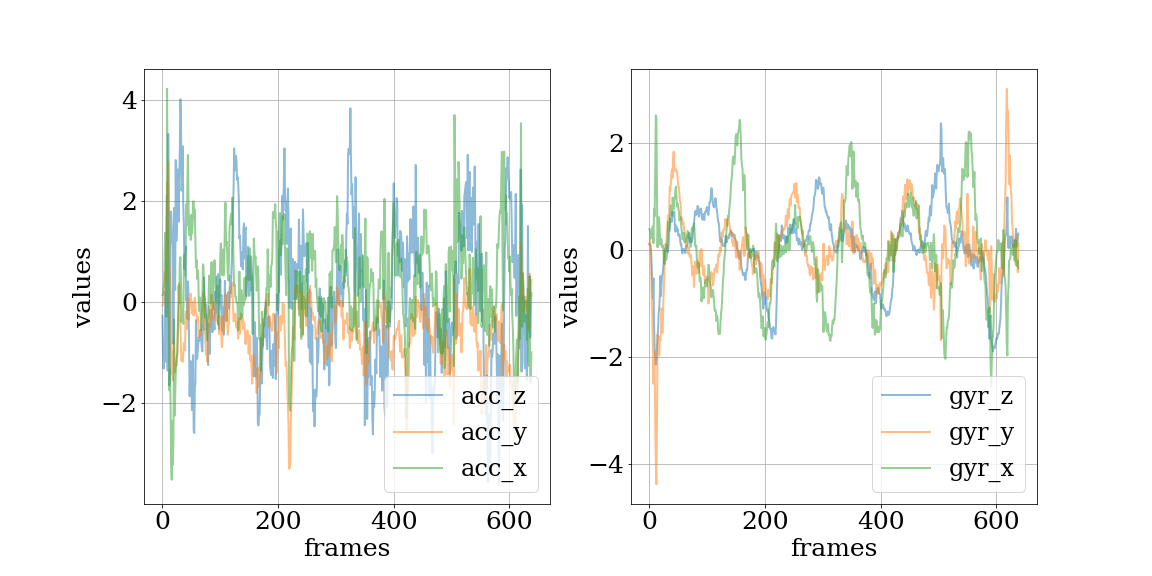
\includegraphics[width=\textwidth]{cyclic_devices_data.png}
	\caption{Данные акселерометра и гироскопа}
	\label{fig:devices_data}
\end{figure}
Первоначальные данные представляют собой набор видеороликов, на которых выполняются различные движения руками (циклические и хаотические), а также показания акселерометра и гироскопа частотой в 100 Герц, закреплённых на одной из рук. 
Далее по видеоряду с помощью фреймворка alphapose \citep{alphapose_fang2017rmpe, alphapose_li2018crowdpose, alphapose_xiu2018poseflow} получаются координаты конечностей, а именно 68 ключевых точек. 
Затем из полученного временного ряда исключаются сильно скореллированные компоненты.
После этого полученные многомерные временные ряды приводятся к одной временной шкале с помощью удаления элементов более длинного временного ряда.

Перед началом эксперимента зафиксируем следующие переменные: $N$ ~--- размерность траекторного пространства, $k$ ~--- число ближайших соседей, рассматриваемых в CCM, $n_{tr}$ ~--- размер обучающей выборки, $E_{vid}$ ~--- число признаков, полученных из видео-ряда, которые будут использованы в алгоритме.
Для каждой пары компонент, взятых из разных временных рядов, применим метод CCM.
В результате получим матрицу корреляций, в которой на $i\text{-ой}$ строке и $j\text{-ом}$ столбце стоит коэффициент корреляции Пирсона между $i\text{-ой}$ компонентной "приборного" временного ряда и $j\text{-ой}$ компонентой ряда, восстановленного по видео. 
После этого для каждого целевого признака выбираем $E_{vid}$ видео-признаков, обладающих максимальной корреляцией в соответствующей строке.
Затем на основе этих признаков обучается алгоритм.

\begin{figure}[bhtp]
	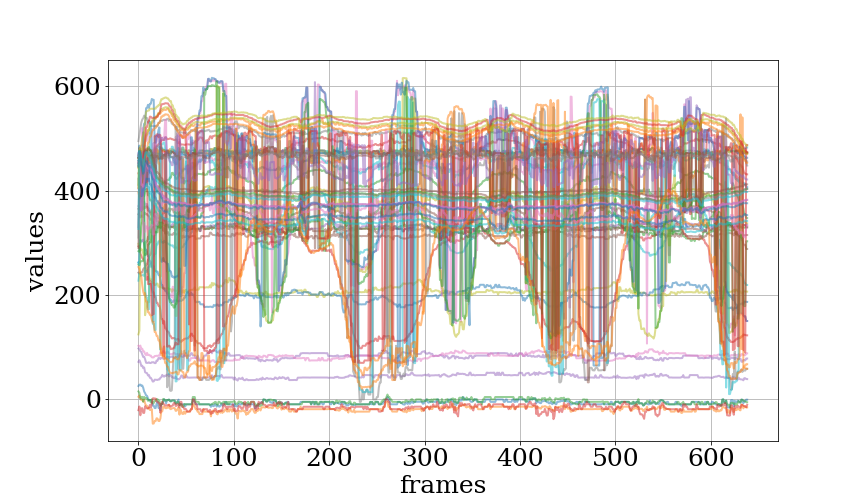
\includegraphics[width=\textwidth]{cyclic_video_data.png}
	\caption{Данные кейпоинтов, полученные по видео}
	\label{fig:video_data}
\end{figure}

\section{Анализ ошибки}
\begin{table}[bhtp]
	\fontsize{10pt}{14pt}
	\selectfont
	\centering
	\caption{Сравнение ошибки (MSE) предсказательной модели, применённой в траекторном пространстве и в его подпространстве, полученном CCM}
	\label{tbl:space_and_subspace}
	\begin{tabularx}{\textwidth}{c|XXXXXX}
		\hline
		& acc\_z & acc\_y & acc\_x & gyr\_z & gyr\_y & gyr\_x \\
		\hline
		space & 1.053 $\pm$ 2.223 & 0.401 $\pm$ 0.833 & 0.483 $\pm$ 0.825 & 0.084 $\pm$ 0.537 & 0.090 $\pm$ 0.094 & 0.063 $\pm$ 0.295 \\
		subspace & 0.315 $\pm$ 0.461 & 0.043 $\pm$ 0.051 & 0.150 $\pm$ 0.177 & 0.001 $\pm$ 0.001	& 0.015 $\pm$ 0.031 & 0.001 $\pm$ 0.003 \\
		\hline
	\end{tabularx}
\end{table}

Для начала сравним качество предсказаний прогностической модели, применённой в траекторном пространстве и его подпространстве.
В таблице \ref{tbl:space_and_subspace} представлены среднеквадратичная ошибки предсказаний значений акселерометра и гироскопа по каждой из осей и их стандартные отклонения. 
На ней видно, что прогностическая модель, применённая в траекторном подпространстве, даёт более точные предсказания, поскольку большинство признаков исходного признакового пространства неинформативно.

Далее, рассмотрим различные методы снижения размерности траекторного пространства. В таблице \ref{tbl:methods} видно, что добавление данных из видеоряда повышает качество модели предсказания.

\begin{table}[bhtp]
	\centering
	\caption{Среднеквадратичное отклонение между истинными показаниями устройств и предсказаниями, полученными с помощью одного из методов снижения размерности}
	\label{tbl:methods}
	\begin{tabular}{l|c|llll}
		\hline
		\multicolumn{2}{l}{\diaghead{\hskip4cm}{Целевой признак}{Метод}} \vline & CCM & PLS & CCA & Naive \\
		\hline
		\multirow{6}{*}{\rotatebox[origin=c]{90}{cyclic}} & acc\_z & 0.163 & \textbf{0.040} & 0.116 & 0.141 \\
		& acc\_y & 0.009 & \textbf{0.007} & 0.011 & 0.008 \\
		& acc\_x & \textbf{0.044} & 0.045 & 0.089 & 0.049 \\
		& gyr\_z & \textbf{0.000} & 0.001 & 0.001 & 0.001 \\
		& gyr\_y & \textbf{0.002} & 0.004 & 0.005 & 0.003 \\
		& gyr\_x & 0.009 & 0.004 & 0.004 & \textbf{0.003} \\
		\hline
		\multirow{6}{*}{\rotatebox[origin=c]{90}{chaotic}} & acc\_z & \textbf{0.315} & 0.416 & 0.416 & 0.331 \\
		& acc\_y & \textbf{0.043} & 0.045 & 0.429 & 0.055 \\
		& acc\_x & 0.150 & 0.177 & 0.221 & \textbf{0.143} \\
		& gyr\_z & \textbf{0.001} & 0.002 & 0.003 & 0.003 \\
		& gyr\_y & \textbf{0.015} & 0.022 & 0.061 & 0.026 \\
		& gyr\_x & \textbf{0.001} & 0.013 & 0.015 & 0.008 \\
		\hline   
	\end{tabular}
\end{table}

\section{Заключение}
В работе предложен метод обобщения методов PLS и CCA с помощью метода Сугихары путём построения эмбеддингов и выбора метрики для оценки качества аппроксимации.  
Проведён вычислительный эксперимент на данных устройств и видеоряда. 
Получено, что использование данных из видео повышает качество прогнозирования. 
Показано, что прогностическая модель менее устойчива в случае, когда та применяется в траекторном пространстве

\bibliographystyle{unsrtnat}
\bibliography{Vladimirov2022RestoringHandMovement.bib}

\end{document}